\documentclass{standalone}
\usepackage{tikz}
\usepackage{amsmath}
\begin{document}

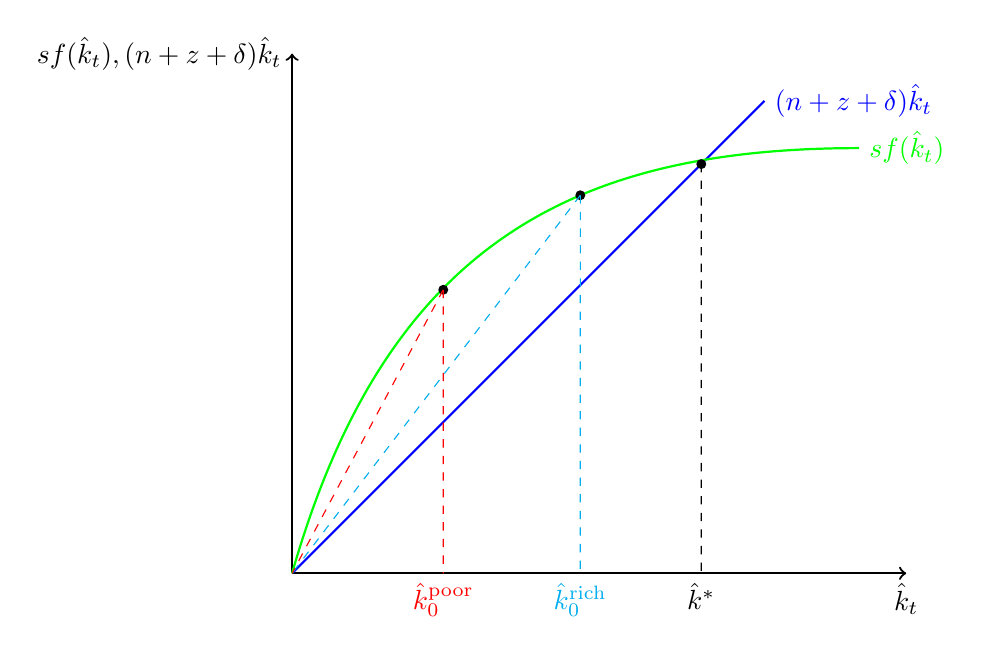
\begin{tikzpicture}[scale=1.2, domain=0:6]
  % Axes
  \draw[thick, ->] (0,0) node[below left] {} -- (6.5,0) node[below] {$\hat{k}_{t}$};
  \draw[thick, ->] (0,0) -- (0,5.5) node[left] {$sf(\hat{k}_{t}), (n+z+\delta)\hat{k}_{t}$};

  % Depreciation line ( \delta k )
  \draw[thick, blue] (0,0) -- (5,5) node[right] {$(n+z+\delta)\hat{k}_{t}$};

  % Saving curve ( sf(k) )
  \draw[thick, green] (0,0) .. controls (1,3.5) and (3,4.5) .. (6,4.5) node[right] {$sf(\hat{k}_{t})$};

  % Steady state markers
  \coordinate (SS) at (4.33, 4.33);
  \coordinate (rich) at (3.05, 4);
  \coordinate (poor) at (1.6, 3);
  \fill[black] (SS) circle (1.5pt);
  \fill[black] (rich) circle (1.5pt);
  \fill[black] (poor) circle (1.5pt);
  \draw[dashed] (SS) -- (4.33,0) node[below] {$\hat{k}^*$};
  \draw[cyan, dashed] (rich) -- (3.05,0) node[below] {$\hat{k}^\text{rich}_0$};
  \draw[cyan, dashed] (rich) -- (0,0);
  \draw[red, dashed] (poor) -- (1.6,0) node[below] {$\hat{k}^\text{poor}_0$};
  \draw[red, dashed] (poor) -- (0,0);
\end{tikzpicture}

\end{document}